\begin{abstract}
	On the MSc course "\textit{Computer Modelling Laboratory}" at ELTE, I've worked on a project in nuclear physics, where I studied the behaviour of the Japanese NEBULA detector when it was bombarded by neutron beams. For the simulation and analysis I've used the Geant4 general-purpose software, which is capable of producing state-of-the-art simulations and results in almost any field in nuclear- or particle physics.
\end{abstract}

\begin{multicols}{2}
\section{Introduction}
At the midterm report I've discussed all of my final considerations and plans for this project until the end of the semester. In the midterm presentation I've then talked about my plans and goals I want to achieve until the next (this) biweekly presentation.

This last two weeks consisted of the implementation of all the remaining technical aspects of the project I planned to do. In more detail, the NEBULA detector rods wasn't able to measure the deposited energy of the inbound neutrons, also the I/O of the data from measurements wasn't yet implemented. However in the last two weeks I've implemented all of them at once.

\section{Making NEBULA rods sensitive for neutrons}
\subsection{Theoretical background}
The key component of the pipeline I've worked on in the last two weeks was to make the already implemented NEBULA rods to be able to measure the deposited energy of transiting neutrons. This capability makes the detector rods inherently "detectors" as they're used in reality. Neutrons sometimes interact with the material inside the detector (which is the BC-$408$ plastic scintillator material in case of the NEBULA detector), which interaction usually involves the release of energy in the form of photons and other particles, such as electrons or protons.

Since we're speaking about a detector operating on the principle of scintillation here, my analysis will be revolve around the study of the released photons. These photons are immediately absorbed by the scintillator material and the system gives off an electric impulse proportionate to its energy. That's why we're usually refer to this as "the deposited energy". Measuring the distribution of this energy in the detector rods and identifying peaks in their spectrum, along with counting the total number of events per rods, we can draw conclusions about the event that created these neutrons.

\subsection{In practice}
As I've consistently emphasized in all of my reports and presentations, Geant4 is the fourth iteration of a several decades old software toolkit, its origins tracing back to the early $1970$s. Hundreds of people worked on the software in the last decades and it is still in constant development as of now in $2021$.

Because of this, Geant4 has a heavily bloated source code, which makes it much more challenging to learn using it. Its concept of serving as a full-fledge engine for application developers instead of eg. simply being a parametrizable tool makes its learning curve even much steeper, than other simulation software.

In previous documents I've already covered the basic principles and aspects of creating a Geant4 simulation. Using those informations here I'll cover what other methods did I use on top of the mentioned ones in the previous two weeks.

During a simulation, Geant4 tracks every particles individually in several steps. At each step its position, mother volume, kinetic energy and other attributes are stored by Geant4. This generally makes the user able to gather the lost/gained energy of each particle in any volumes it passes during a simulation. In my case, I've collected the energy deposited by each event in each rod individually.

This was done by assigning a \texttt{G4Accumulable} object to each detector rod. When a particle entered a rod - marked with the identifier \texttt{CounterX} (where \texttt{X} is a number ID from $1$ to $20$ corresponding to every one of the $20$ rods in total) -, it first checked which \texttt{G4LogicalVolume} is assigned to this rod. Then the energy deposited by the particle in this volume was added to the corresponding \texttt{G4Accumulable} object. After the particle reached the end of its lifetime by exiting the \texttt{World} volume of the simulation, the energy values for each rod was written to an output file, where each columns correspond to the different rods and each row corresponds to different instances/neutrons. Because neutrons usually interacted with $1$, of maximally $2$ rods during their lifetime, most of the columns contain zeros for each instances. At the end of a full simulation with $N$ number of neutrons, we obtained a dataset in the size of $20 \times N$ entries. In summary, an entry in the $M$th row and $X$th column corresponds to the energy deposited by the $M$th neutron in the $X$th NEBULA detector rod.

\section{The \texttt{G4Analysis} pipeline}
Geant4 has no built-in post-processing tools, which means one has to use some other, third-party software to visualize and analyse data accumulated in a simulation. For this, Geant4 offers a versatile I/O library that is able to save any data in the form of XML, CSV or ROOT format.

The \texttt{G4AnalysisManager} is single-handedly responsible for the creation, filling and finally saving the data storing objects in Geant4. As mentioned in the previous section, each dataset consisted of $20$ columns, each column representing a unique detector rod. At the start of a run, the analysis manager object was created and assigned $20$ columns to the dataset. As it was also previously mentioned, at the end of each event (each particle tracing) the values of the $20$ \texttt{G4Accumulable} objects was added to the dataset. After all $N$ number of events were finished, the dataset was saved to disk in a \texttt{csv} format file in my case.

Any further analysis was done using \texttt{Python 3.9} using the created datasets as input for them.

\section{Exploration of the output data}
I'm admittedly have little to none expertise in modern nuclear physics besides those things I've learned on the university. Therefore during the analysis I've mostly concentrated on data exploration instead of the explanation of the obtained results. I've made simulation runs with a $N = 100$ and $N = 1000$ particles on $E = 20$ Mev, $E = 100$ MeV, $E = 200$ MeV and $E = 300$ MeV energies.
\begin{Figure}
	\centering
	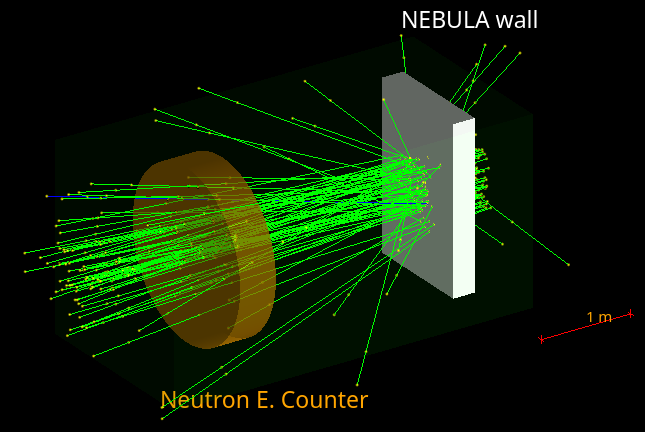
\includegraphics[width=\linewidth]{{images/nebula_3d.png}}
	\captionof{figure}{Particle traces penetrating the NEBULA detector after a neutron run of $100$ neutrons of $100$ MeV in the OpenGL+Qt visualization of the Geant4 simulation.} \label{fig:1}
\end{Figure}
As seen on Figures \ref{fig:2} - \ref{fig:5}, the smaller the energy of a neutron, the earlier it absorbed by the detector material. While the larger its energy get, the detector stops it with a smaller probability. That's the reason why the NEBULA detector operates in the $100-300$ MeV energy range. Smaller energies are absorbed at the first column and makes particle tracing impossible. Particles with larger energies however penetrates the whole detector system with almost zero interaction and thus with very low detection rate.

A different visualization of the same thing can be seen on Figures \ref{fig:6} - \ref{fig:9}, where the distribution of the deposited energies are visualized for each detector rod.

Particle tracing is a built-in feature of Geant4 as seen on the Figure \ref{fig:1}. The particle traces of neutrons are marked with green lines, while occasionally created electrons in the detector are marked with with blue coloured lines.

\begin{figure*}
	\captionsetup{font={normalsize}}
	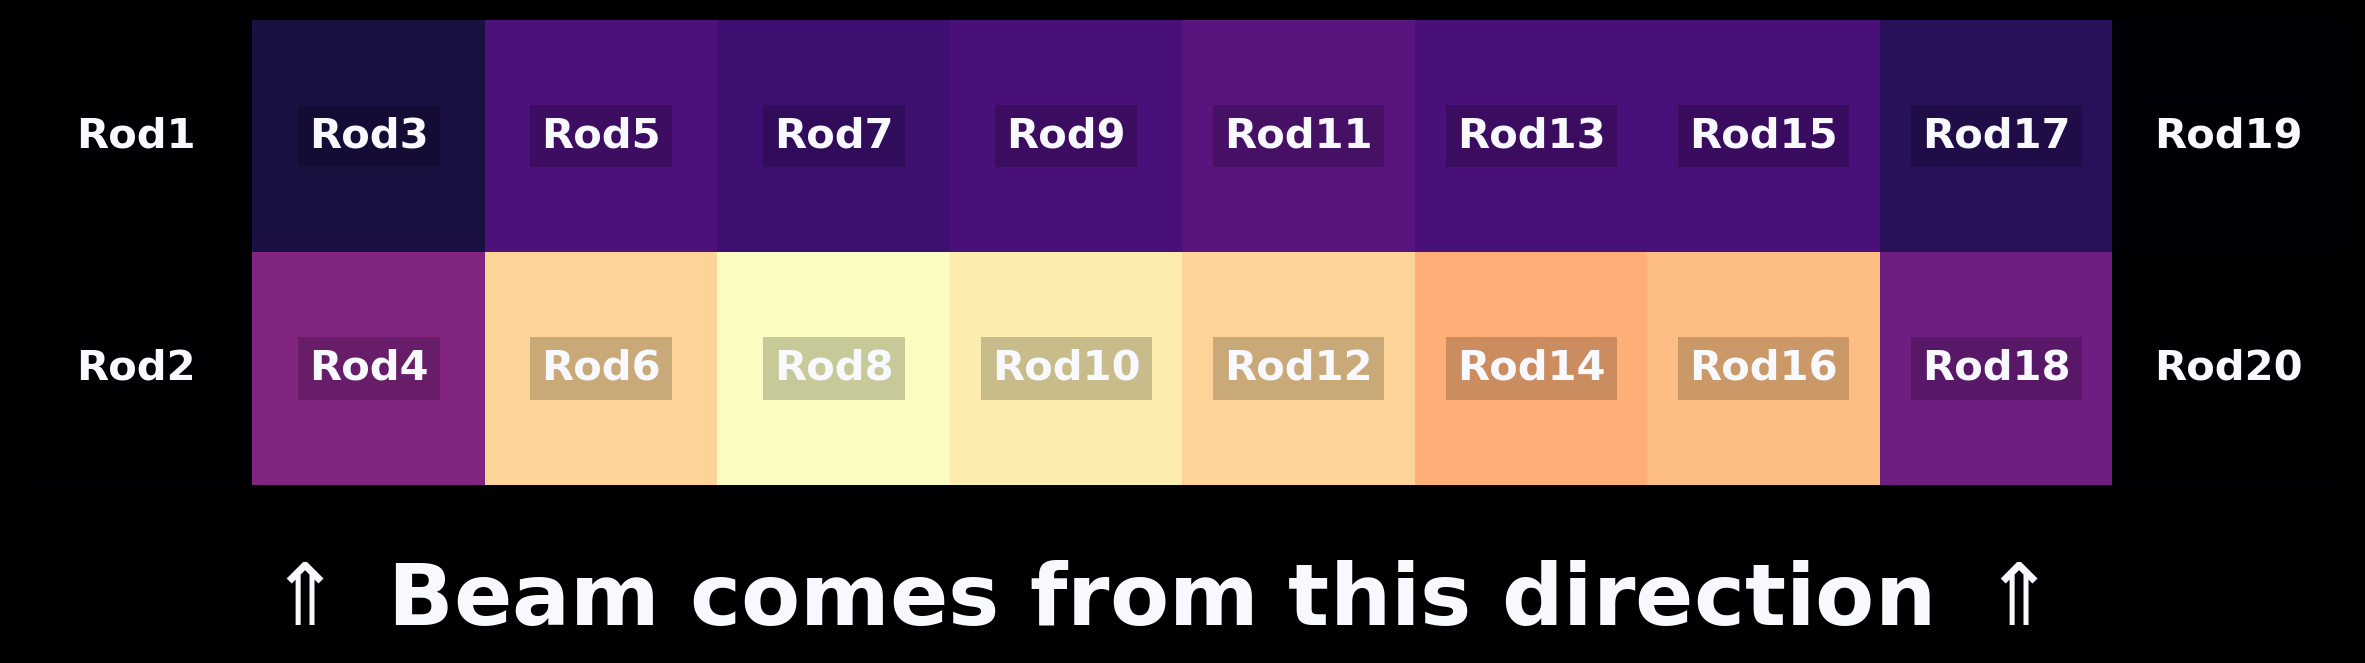
\includegraphics[width=\textwidth]{{images/rod_heatmap_20.png}}
	\captionof{figure}{Heatmap of the total deposited energy in the NEBULA detector rods during a test run of $1000$ neutrons of $20$ MeV.}\label{fig:2}
\end{figure*}
\begin{figure*}
	\captionsetup{font={normalsize}}
	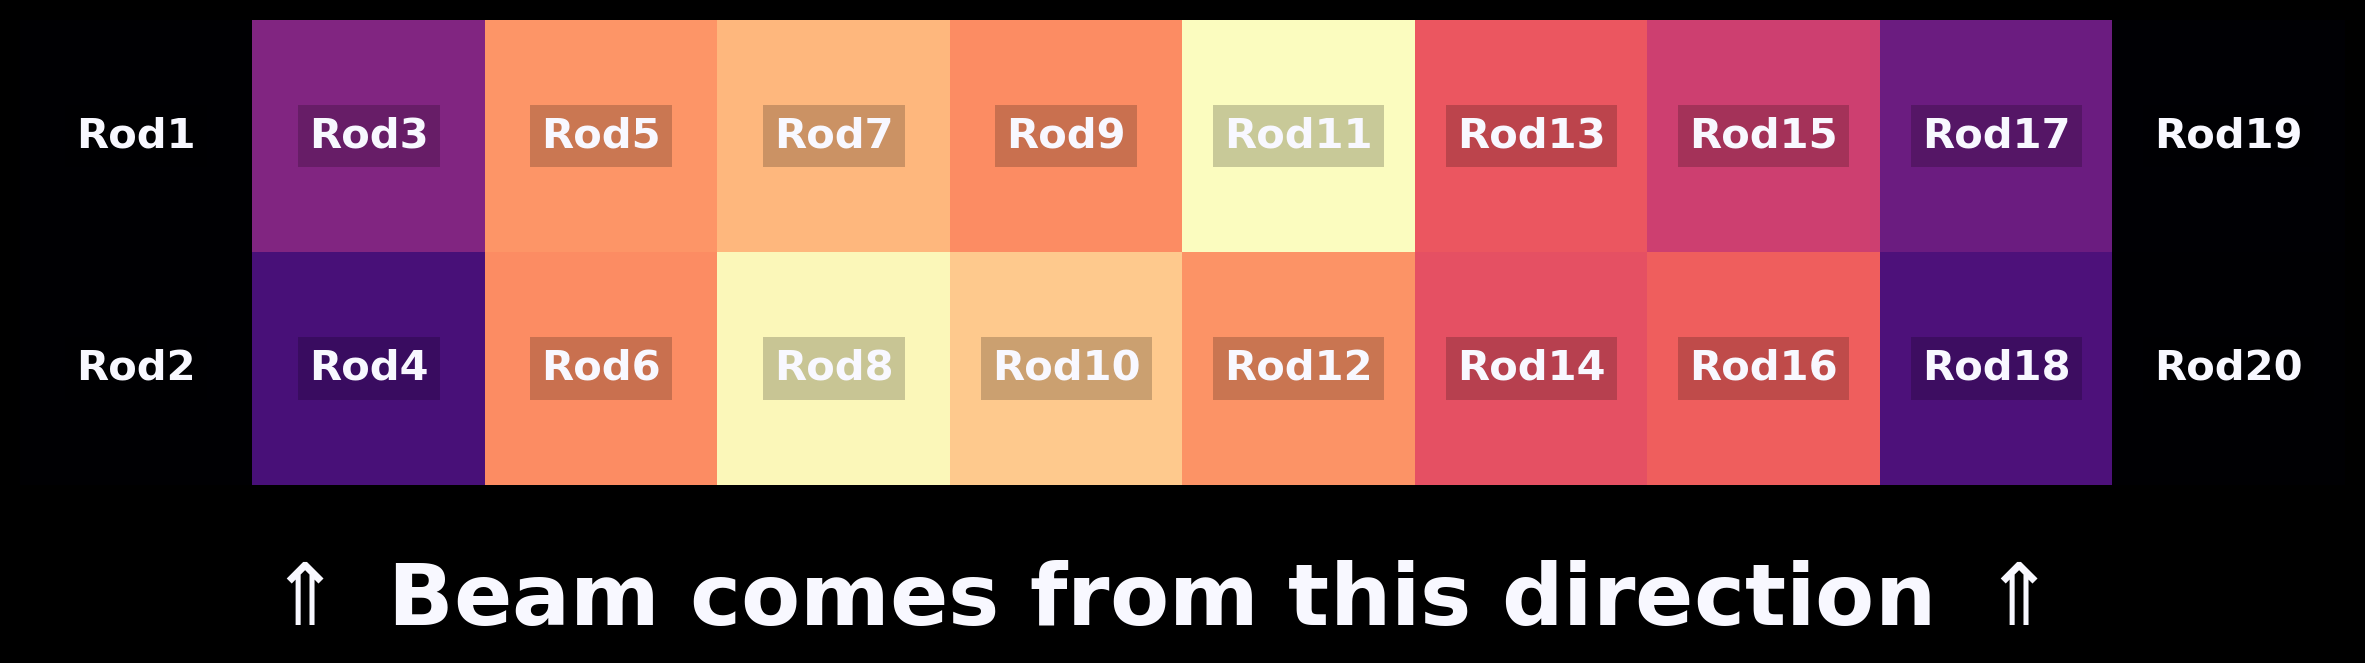
\includegraphics[width=\textwidth]{{images/rod_heatmap_100.png}}
	\captionof{figure}{Heatmap of the total deposited energy in the NEBULA detector rods during a test run of $1000$ neutrons of $100$ MeV.}\label{fig:3}
\end{figure*}
\begin{figure*}
	\captionsetup{font={normalsize}}
	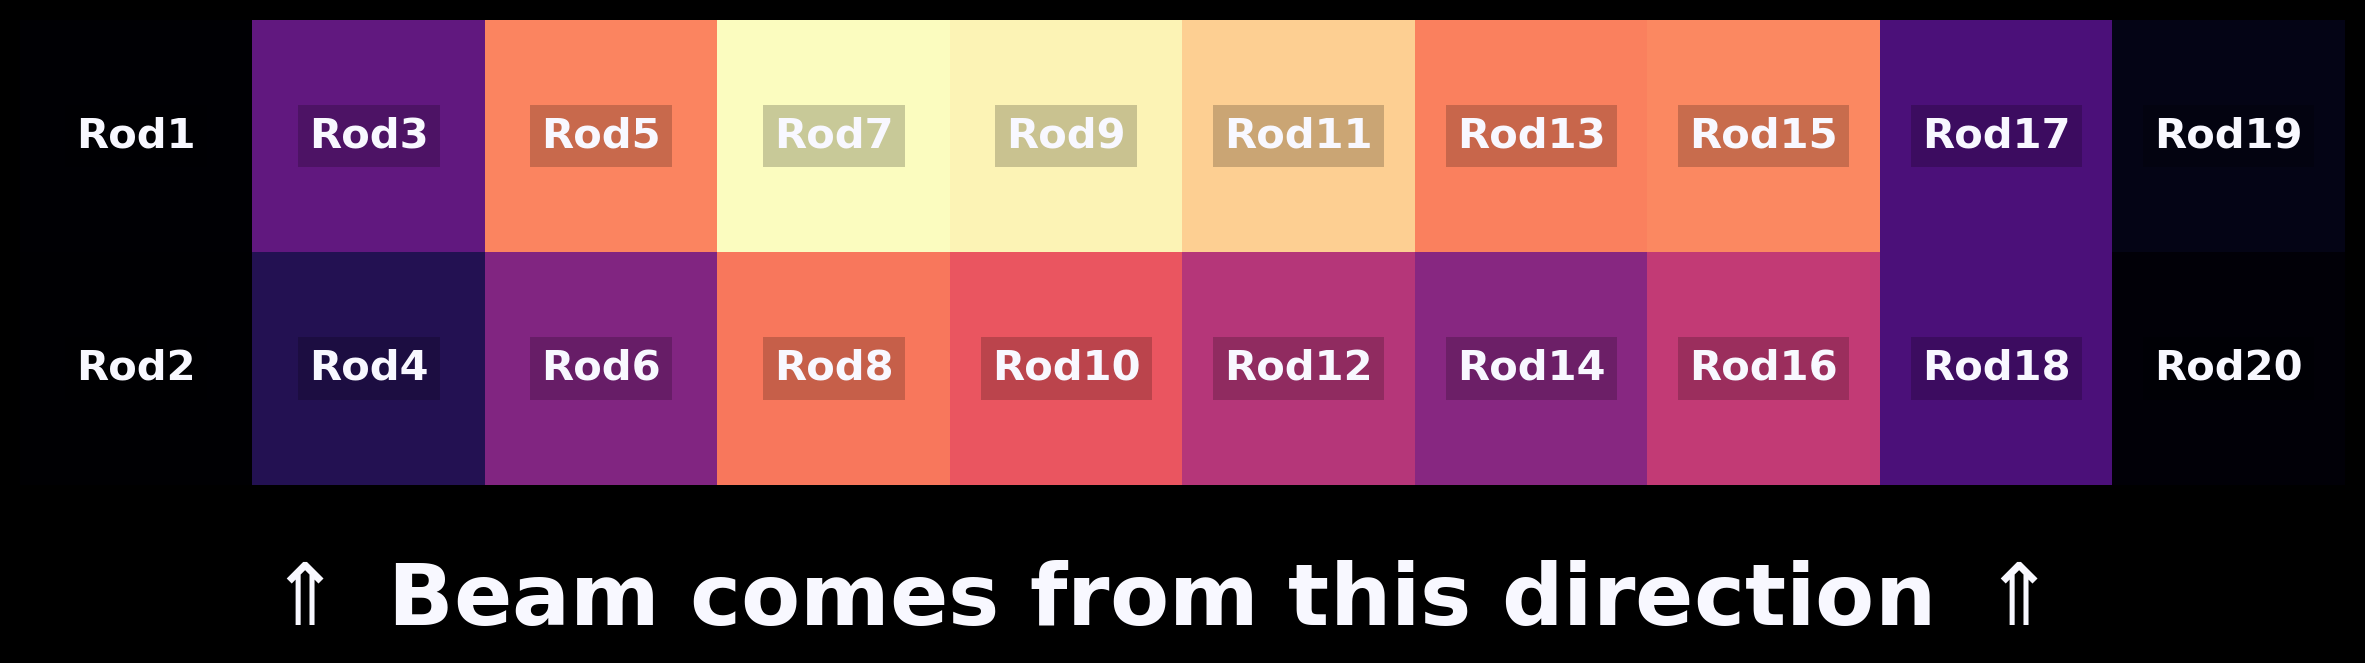
\includegraphics[width=\textwidth]{{images/rod_heatmap_200.png}}
	\captionof{figure}{Heatmap of the total deposited energy in the NEBULA detector rods during a test run of $1000$ neutrons of $200$ MeV.}\label{fig:4}
\end{figure*}
\begin{figure*}
	\captionsetup{font={normalsize}}
	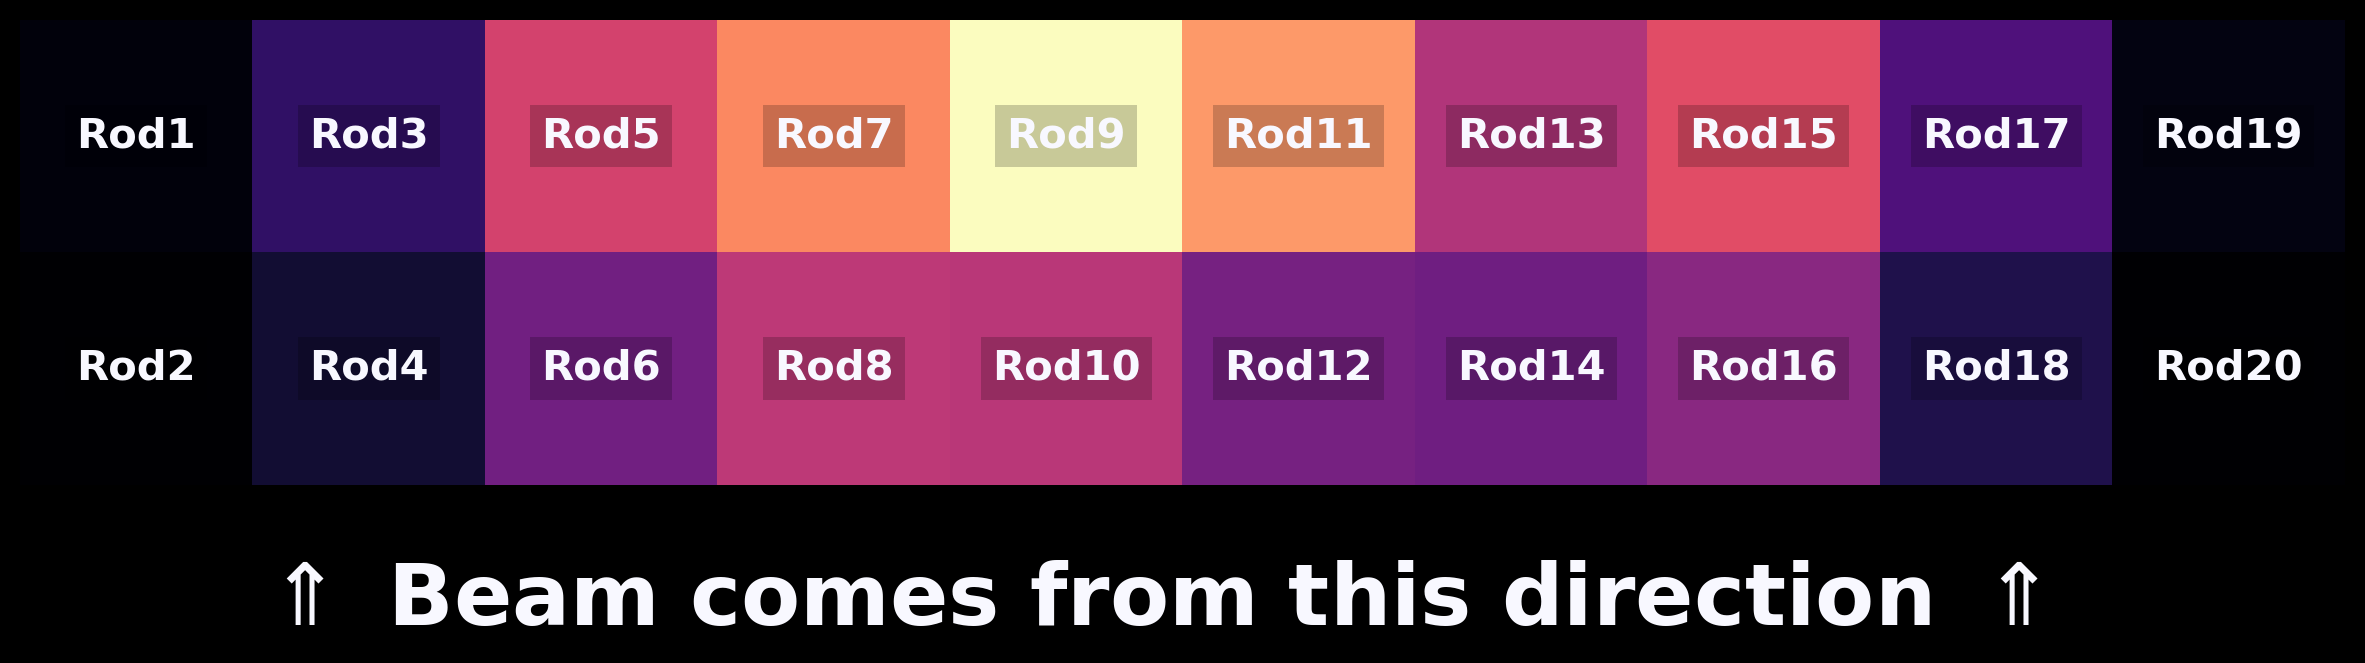
\includegraphics[width=\textwidth]{{images/rod_heatmap_300.png}}
	\captionof{figure}{Heatmap of the total deposited energy in the NEBULA detector rods during a test run of $1000$ neutrons of $300$ MeV.}\label{fig:5}
\end{figure*}

\begin{figure*}
	\captionsetup{font={normalsize}}
	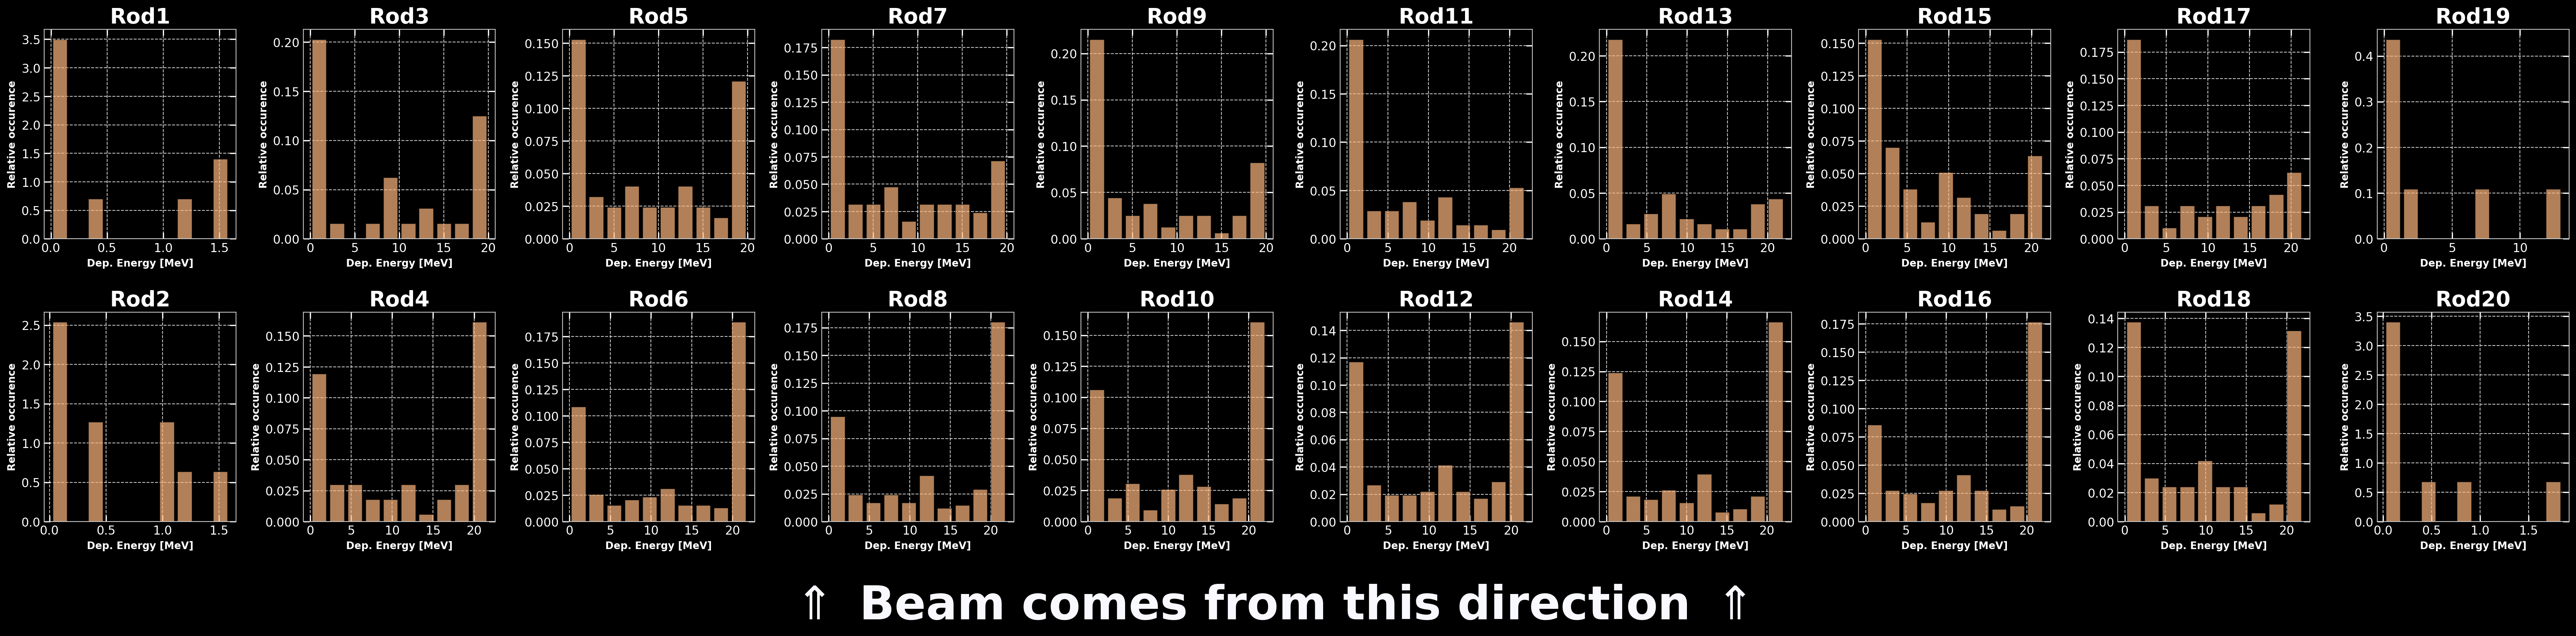
\includegraphics[width=\textwidth]{{images/energy_dist_per_rod_20.png}}
	\captionof{figure}{Histogram of the deposited energies for each NEBULA detector rods during a test run of $1000$ neutrons of $20$ MeV.}\label{fig:6}
\end{figure*}
\begin{figure*}
	\captionsetup{font={normalsize}}
	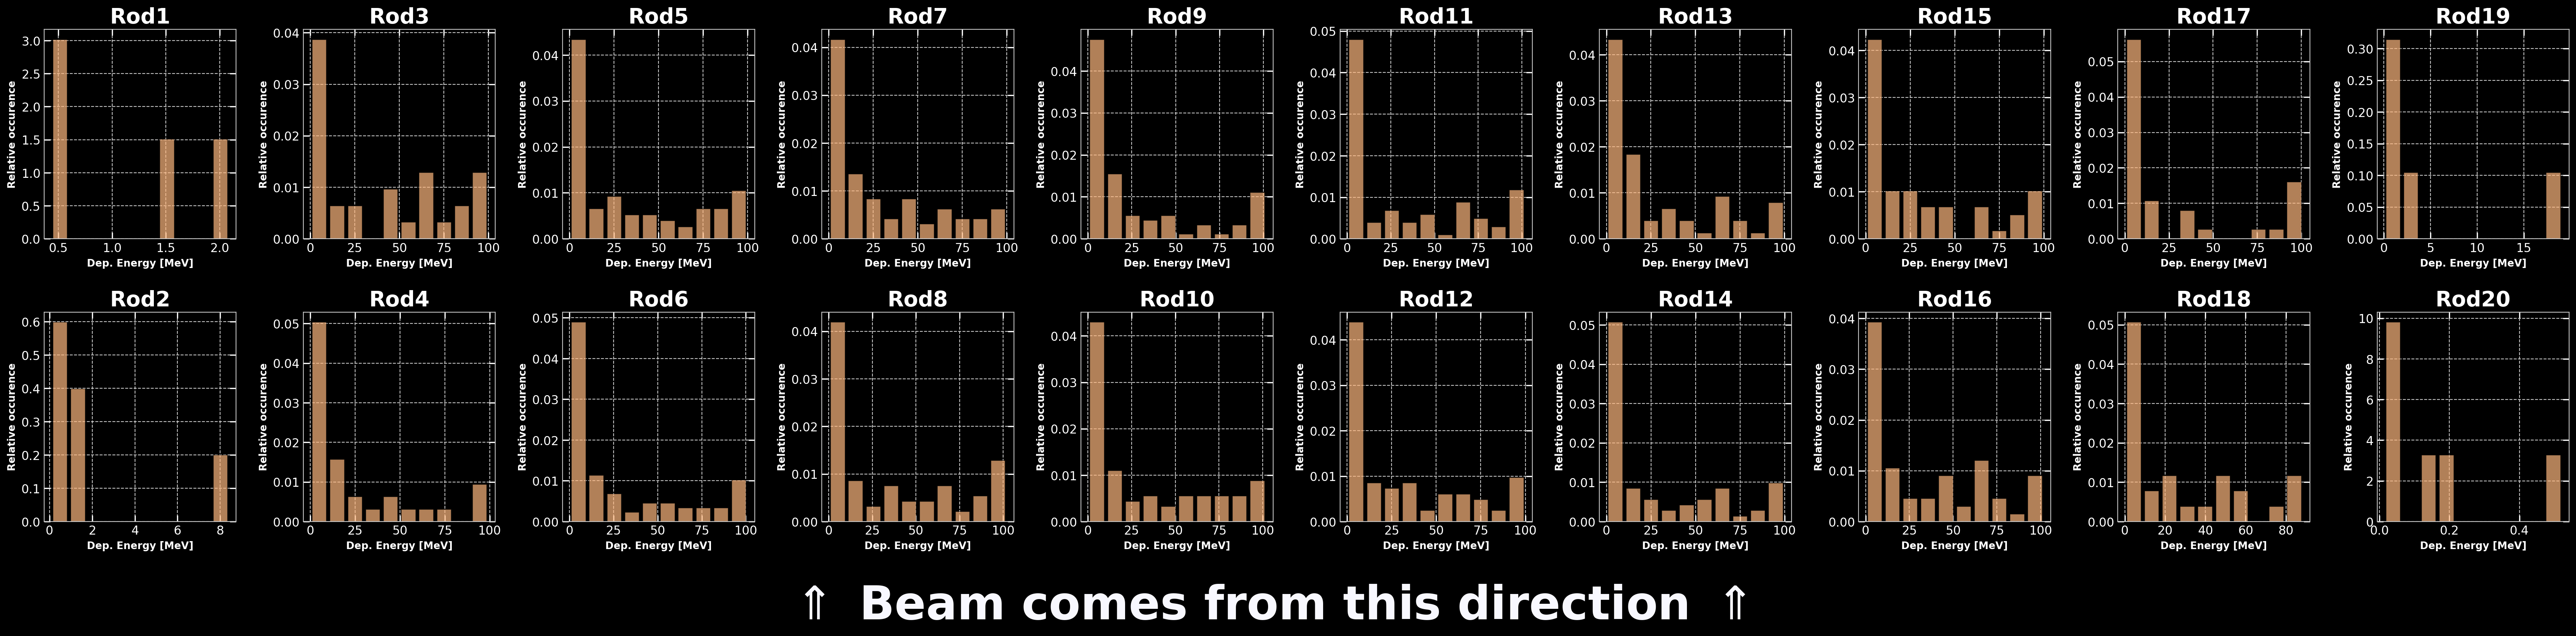
\includegraphics[width=\textwidth]{{images/energy_dist_per_rod_100.png}}
	\captionof{figure}{Histogram of the deposited energies for each NEBULA detector rods during a test run of $1000$ neutrons of $100$ MeV.}\label{fig:7}
\end{figure*}
\begin{figure*}
	\captionsetup{font={normalsize}}
	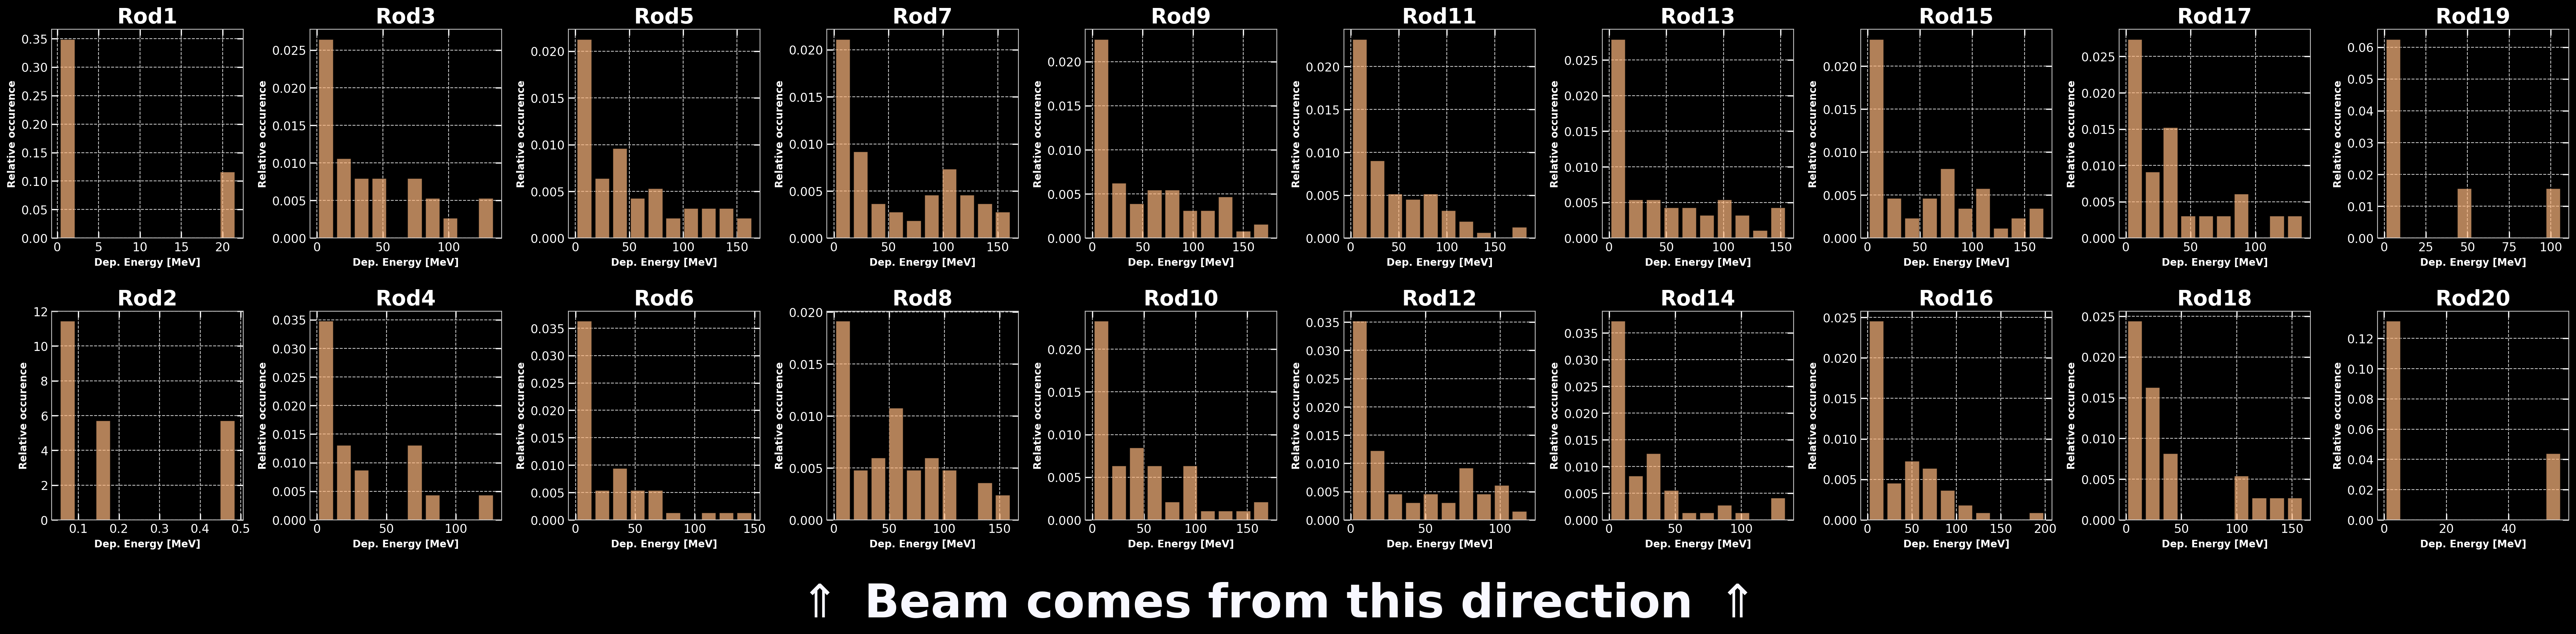
\includegraphics[width=\textwidth]{{images/energy_dist_per_rod_200.png}}
	\captionof{figure}{Histogram of the deposited energies for each NEBULA detector rods during a test run of $1000$ neutrons of $200$ MeV.}\label{fig:8}
\end{figure*}
\begin{figure*}
	\captionsetup{font={normalsize}}
	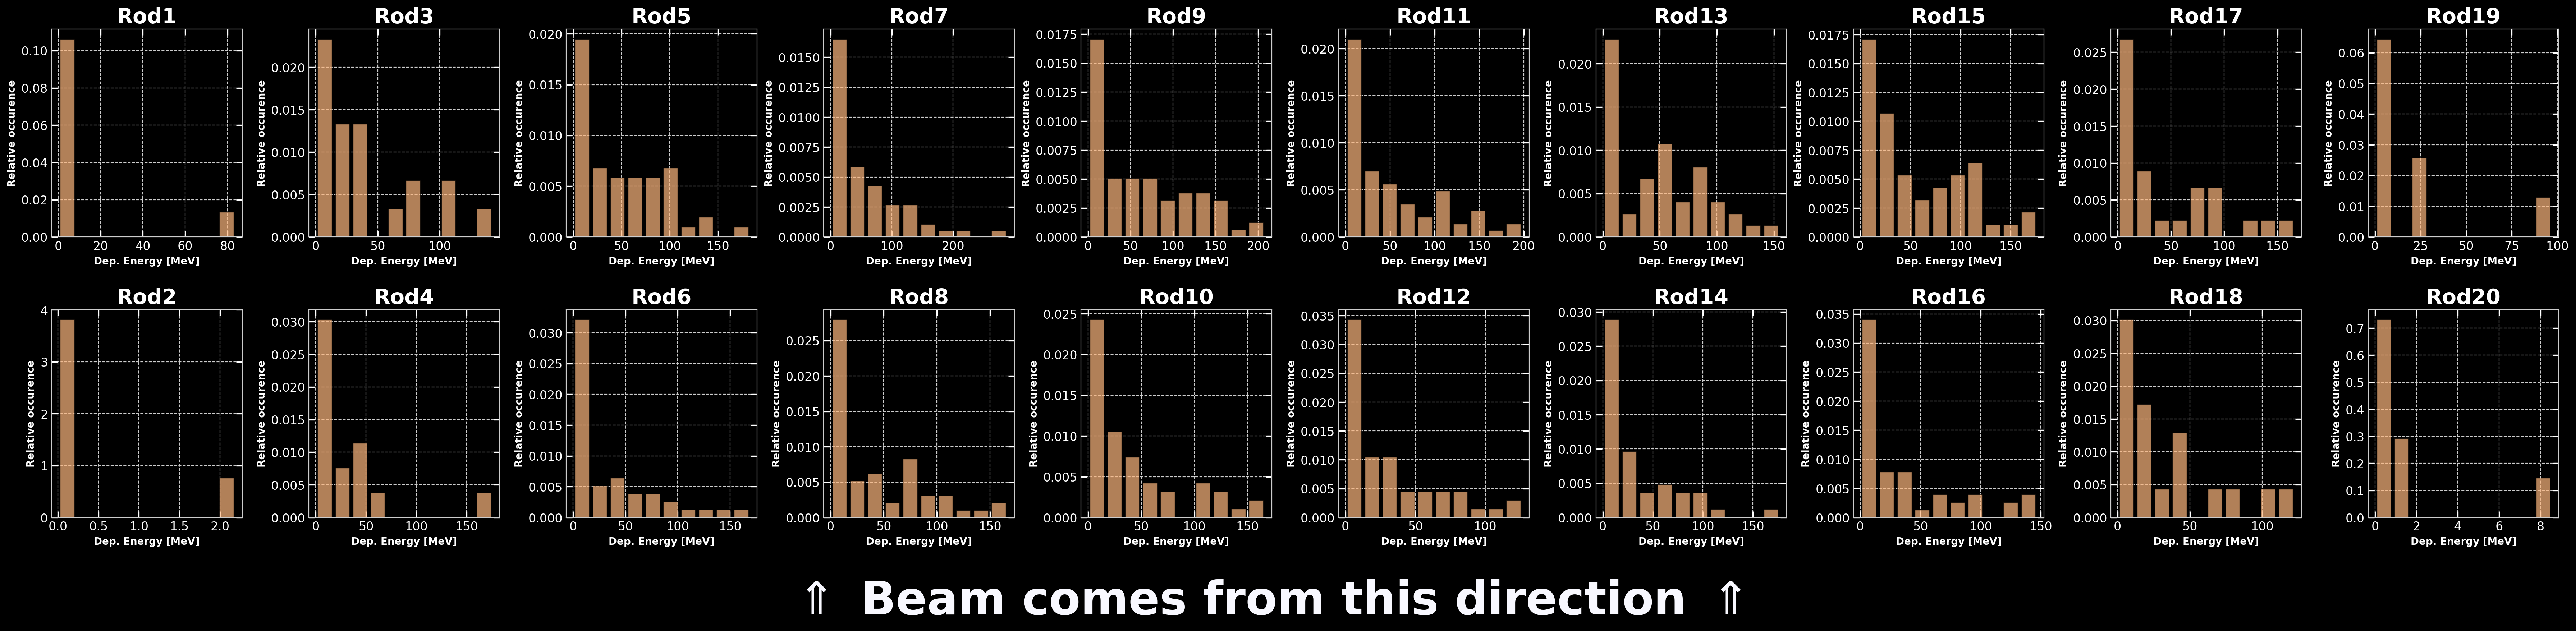
\includegraphics[width=\textwidth]{{images/energy_dist_per_rod_300.png}}
	\captionof{figure}{Histogram of the deposited energies for each NEBULA detector rods during a test run of $1000$ neutrons of $300$ MeV.}\label{fig:9}
\end{figure*}

\section{Plans for next week}
The next and probably final step in the project will be to test the now finalized NEBULA pipeline for some of the pre-defined particle beams of real physical processes. If expected results are obtained from these test, it will assure, that the whole pipeline was finished and works as it supposed to be.
\end{multicols}